% !TEX program = pdflatex
% Reviewer-response status presentation
% Audience: paper team + tracking-tech (non-LHCb) collaborators
% Target length: 10-15 min
\documentclass[aspectratio=169]{beamer}

\usepackage[T1]{fontenc}
\usepackage{lmodern}
\usepackage{amsmath, amssymb}
\usepackage{graphicx}
\usepackage{booktabs}
\usepackage{xcolor}
\usepackage{tikz}

\providecommand{\ket}[1]{\left|#1\right\rangle}
\providecommand{\bra}[1]{\left\langle#1\right|}
\providecommand{\braket}[1]{\left\langle#1\right\rangle}

\IfFileExists{beamerthememetropolis.sty}{\usetheme{metropolis}}{\usetheme{Madrid}\usecolortheme{seahorse}}
\setbeamertemplate{caption}{\insertcaption}
\setbeamerfont{footnote}{size=\tiny}

% Tighter typography to fit more on each slide
\AtBeginDocument{\small}
\setbeamerfont{frametitle}{size=\normalsize,series=\bfseries}
\setbeamerfont{itemize/enumerate body}{size=\small}
\setbeamerfont{itemize/enumerate subbody}{size=\footnotesize}
\setbeamerfont{itemize/enumerate subsubbody}{size=\scriptsize}
\setbeamertemplate{itemize items}[circle]
\setlength{\leftmargini}{1.2em}
\setlength{\leftmarginii}{1.0em}
\setbeamersize{text margin left=4mm,text margin right=4mm}

\graphicspath{%
  {/data/bfys/gscriven/Quantum_Track_Reconstruction/Toy_Characterisation/Verify_new_results/outputs/segment_analysis/paper/}%
  {/data/bfys/gscriven/Quantum_Track_Reconstruction/Toy_Characterisation/Verify_new_results/outputs/segment_analysis/}%
}

\newcommand{\openflag}[1]{{\color{orange}\textbf{[open: #1]}}}
\newcommand{\done}{{\color{teal}\textbf{[done]}}}

\title{Paper review progress}
\author{George Scriven \and Xenofon Chiotopoulos}
\institute{\small \emph{Communications Physics} resubmission — detailed responses live in the Overleaf answer file.}
\date{29 April 2026}

\begin{document}

\maketitle

% =====================================================================
\begin{frame}{Outline}
\begin{enumerate}
  \item Recap of the paper
  \item Reviewer overview
  \item Major comments and our planned responses
  \item Minor comments
  \item New benchmarks supporting the response
  \begin{itemize}
    \item Toy --- classical (George): \textbf{ready}; quantum (George): \textbf{preliminary results ready}
    \item Realistic LHCb MC (Xeno): \textbf{in progress}
    \item Hardware/emulator (Xeno): \textbf{ready}
  \end{itemize}
  \item Open items \& schedule
  \item Extras --- track-level metrics and tracker A/B
\end{enumerate}
\end{frame}

% =====================================================================
\section{Recap}

\begin{frame}{What the paper proposes}
\textbf{1-Bit Quantum Filter} for particle-track reconstruction:
\begin{itemize}
  \item Reformulates HHL: from \emph{matrix inversion} to \emph{spectral filtering}.
  \item The track-finding Hamiltonian collapses combinatorial-noise eigenstates onto a known eigenvalue $\lambda_c$.
  \item One ancilla qubit + a single phase-rotation step projects them out; signal eigenstates pass through with a $\cos^2(\lambda_j t/2)$ response.
\end{itemize}
\smallskip
\textbf{Circuit complexity} (\,$N$ = matrix size = segment-pair count\,)
\begin{itemize}
  \item \textbf{Direct Structural Synthesis} replaces Trotterisation $\Rightarrow$ $\mathcal{O}(\sqrt{N}\log N)$ gates.
  \item Demonstrations on emulators of three QPU architectures (Quantinuum H2, IBM-Fez, IBM-Pittsburgh).
\end{itemize}
\end{frame}

% =====================================================================
\section{Reviewer overview}

\begin{frame}{Three reviewers --- big picture}
\begin{itemize}
  \item \textbf{Reviewer 1} --- co-review notice only, no scientific content.
  \item \textbf{Reviewer 2} --- 3 major + 4 minor comments. Critical:
  \begin{itemize}\footnotesize
    \item Classical alternatives + $\mathcal{O}(N)$ load complexity
    \item Realism / model limitations (claim that the method is ``limited to $\le 4$ particles, $\le 3$ layers'')
    \item Generality of the conceptual advance
  \end{itemize}
  \item \textbf{Reviewer 3} --- positive overall:
  \begin{itemize}\footnotesize
    \item Wants HL-LHC context and a fault-tolerant scaling discussion.
    \item Detailed line-by-line edits to Methods + bibliography.
  \end{itemize}
\end{itemize}
\end{frame}

% =====================================================================
\section{Reviewer 2 --- Major comments}

\begin{frame}{R2 Major 1 --- Classical alternatives \& $\mathcal{O}(N)$ load}
\textbf{Concern.} Classical limits are not quantified. $\mathcal{O}(N)$ data loading may erase the quantum speed-up
{\footnotesize (Phys.\ Rev.\ D \textbf{101}, 094015)}.
\smallskip

\textbf{Our response.}
\begin{itemize}
  \item No QRAM / external state preparation: $\ket b$ is loaded by Hadamards, $\mathbf A$ is embedded gate-by-gate by DSS.
  \item Both costs are already inside the $\mathcal{O}(\sqrt{N}\log N)$ count --- no hidden $\mathcal{O}(N)$ load.
  \item An explicit step-by-step paragraph is being added to the Gate Complexity section.\hfill\done
\end{itemize}
\smallskip
\openflag{HL-LHC throughput / classical-limit prose; ``outperform classical'' sentence --- not yet drafted.}
\end{frame}

% =====================================================================
\begin{frame}{R2 Major 2 --- Realism \& limitations}
\textbf{Concern.} Method only shown on straight tracks, $\le 3$ layers, $\le 4$ particles; will it survive realistic detector effects?
\smallskip

\textbf{Clarifications already in the manuscript:}
\begin{itemize}\small
  \item The \emph{toy} model already includes multiple scattering and detector resolution.
  \item The 4-particle / 3-layer ceiling refers to the \emph{quantum-emulation reach} of the manuscript demos, not the algorithm. Statevector simulations already scale to 1000 particles. \hfill\openflag{verify exact limit in the paper}
\end{itemize}
\smallskip

\textbf{New benchmarks:}
\begin{itemize}\small
  \item \textbf{Toy} (George): segment-level classical benchmark up to $n_{\mathrm{trk}}=1000$, with hit-drop test --- ready. Quantum equivalent --- preliminary results up to $n_{\mathrm{trk}}=60$.
  \item \textbf{Realistic MC} (Xeno): 1BQF on the Nicotra et al.\ events (arXiv:2308.00619), benchmarked vs.\ Search-by-Triplet --- in progress.
\end{itemize}
\end{frame}

% =====================================================================
\begin{frame}{R2 Major 3 --- Generality of the conceptual advance}
\textbf{Concern.} The spectral-filter trick may be too tailored to this Hamiltonian.
\smallskip

\textbf{Planned response:}
\begin{itemize}
  \item Within tracking: extends naturally to \textbf{curved tracks} via the original Hamiltonian (Debney/Pearson).
  \item More broadly: any problem where the noise eigenstates collapse onto a single known eigenvalue admits the same one-bit filter --- useful when filtering a specific eigenvalue is enough and full inversion is not required.
\end{itemize}
\smallskip
\openflag{Prose not yet drafted; cross-domain example problems still being identified.}
\end{frame}

% =====================================================================
\section{Reviewer 2 --- Minor comments}
\begin{frame}{R2 Minor comments}
\small
\begin{itemize}
  \item \textbf{Hardware run on a real device.} Planned via Quantinuum + IBM. \openflag{tight in 2 weeks}
  \item \textbf{Eq.\ 6} ($\ket b$ as $\ket+^{\otimes n_s}$). Defined $\ket b = H^{\otimes n_s}\ket 0 = \ket+^{\otimes n_s}$; clarified the eigenbasis form is needed for the next step.\hfill\done
  \item \textbf{Eq.\ 10 intermediate uncomputation step.} Drafted; merge into manuscript pending.
  \item \textbf{Error mitigation.} None used; will state explicitly and flag as future work.
\end{itemize}
\end{frame}

% =====================================================================
\section{Reviewer 3}

\begin{frame}{R3 General comments}
\begin{itemize}
  \item \textbf{At what $N$ does the asymptotic advantage matter for HL-LHC?} Will add an HL-LHC event-size reference line on the complexity figure.
  \item \textbf{HL-LHC timeline in the introduction.} Framed as scaling and dependency on fault-tolerant hardware, not as a single-paper deliverable.
  \item \textbf{Fault-tolerant scaling discussion.} \openflag{short paragraph TBD}
  \item \textbf{Sparsity at HL-LHC.} Refer to Nicotra et al.: matrix sparsity grows at most as $\sqrt{N}$ with event size, which keeps the gate count in the regime claimed.\hfill\done
  \item \textbf{Why PVs / dense observables matter for non-LHCb readers.} Discussion expanded; PV used as a concrete example of an $\mathcal O(1)$-information observable that avoids $\mathcal O(N)$ tomography.\hfill\done
\end{itemize}
\end{frame}

% =====================================================================
\begin{frame}{R3 Line-by-line edits --- summary}
\textbf{$\sim$13 textual edits to Methods + a full bibliography rebuild.}
\smallskip

\textbf{Already done:}
\begin{itemize}\footnotesize
  \item $\theta$ defined before Eq.\ 2; ``positive semi-definite'' remark moved after Eq.\ 9.
  \item $\beta_j \to c_j$ to remove the notation clash with the Hamiltonian's $\beta$.
  \item Repetition removals; Aer wording fix; BW-friendly linestyles in Fig.\ 5.
  \item Fig.\ 4 caption clarifies the ``\#p'' point labels; uncertainty source explained.
  \item Bibliography: DOIs uniform, missing DOIs added, capitalisation fixed.
\end{itemize}
\smallskip

\textbf{Still to do:}
\begin{itemize}\footnotesize
  \item $n_s$ definition; reference for ``classical exhaustive search methods''.
  \item Expansion of the fake-rate discussion (ties into R2 Major 2).
  \item Notation consistency for $r_1, r_2, r_3$.
\end{itemize}
\end{frame}

% =====================================================================
\section{New benchmarks}

\begin{frame}{Toy benchmarks --- what we have and what is coming}
\textbf{Goal:} address R2 Major 2 (``realism / scaling'') by pushing the toy to LHCb-realistic multiplicity, in both the classical and quantum solvers, with realistic detector effects.
\smallskip

\begin{columns}[T]
\column{0.5\textwidth}
\textbf{Classical toy (George) --- ready}
\begin{itemize}\small
  \item Up to $n_{\mathrm{trk}}=1000$
  \item Clean and 1\% hit-drop
  \item Multiple scattering + detector resolution
  \item Segment-level efficiency, false-rate, spectrum
\end{itemize}
\column{0.5\textwidth}
\textbf{Quantum toy (George) --- preliminary}
\begin{itemize}\small
  \item Same setup, run with the 1-bit quantum filter
  \item First direct quantum-vs-classical comparison shown later
  \item Reach so far: $n_{\mathrm{trk}} \le 60$, single noise level
\end{itemize}
\end{columns}
\smallskip
\centering\footnotesize
Following slides show the classical results, then the preliminary quantum comparison.
\end{frame}

% =====================================================================
\begin{frame}{Headline --- segment efficiency \& false rate vs $n_{\mathrm{trk}}$}
\centering

\includegraphics[width=0.85\textwidth,height=0.58\textheight,keepaspectratio,trim=0 0 0 70,clip]{fig14_solver_segment_efficiency_drop1pct_logx.pdf}\\[2pt]
{\scriptsize Classical solver, 1\,\% hit-drop. Segment efficiency stays at $96$--$98\%$ across $n_{\mathrm{trk}}=2$--$1000$.
False-positive segment rate is $<2\%$ up to $n=300$, climbing to $\sim 20\%$ at $n=1000$.
Metrics use the segments \textbf{accepted from the solution vector}, not the geometrically-acceptable set.}
\end{frame}

% =====================================================================
\begin{frame}{Solver-level segment efficiency overlay (clean vs drop=1\,\%)}
\centering

\includegraphics[width=0.85\textwidth,height=0.58\textheight,keepaspectratio,trim=0 0 0 50,clip]{fig14_solver_segment_efficiency_overlay_drop1pct.pdf}\\[2pt]
{\scriptsize The drop=1\% curve tracks the clean curve closely --- the algorithm is robust to small hit inefficiencies.}
\end{frame}

% =====================================================================
\begin{frame}{1-bit quantum filter vs classical solver (preliminary)}
\centering

\includegraphics[width=0.92\textwidth,height=0.58\textheight,keepaspectratio,trim=0 0 0 40,clip]{fig18d_quantum_segment_efficiency_drop1pct.pdf}\\[2pt]
{\scriptsize Segment efficiency (top) and false rate (bottom) for the 1-bit quantum filter (\textbf{Q}, filled circles) and the classical solver (\textbf{C}, open squares) at threshold $\tau{=}0.35$. Clean (blue) vs 1\,\% hit-drop (red), $n_{\mathrm{trk}} = 2{-}60$. \textbf{Caveats:} emulator-only; single noise level; Q efficiency dips at very low $n$ and degrades past $n\sim 30$; Q false rate stays $<0.05\%$ throughout.}
\end{frame}

% =====================================================================
\begin{frame}{What the toy already tells the reviewers}
\textbf{R2 Major 2 --- realism / scaling:}
\begin{itemize}
  \item Algorithm is \textbf{not limited to 4 particles}; the toy goes to 1000 with realistic scattering and resolution.
  \item Survives a 1\% hit-drop without collapse.
  \item The false-positive tail is small, well-characterised, and threshold-tunable.
\end{itemize}
\smallskip
\textbf{R3 --- conditioning \& sparsity:}
\begin{itemize}
  \item Condition number $\kappa$ grows only $\sim 3.4\times$ over two decades of $n_{\mathrm{trk}}$ \emph{(preliminary --- still being tested; correct up to Hamiltonian-diagonal corrections)}.
  \item The true/false separation gap stays clean at every $n$ --- the Hamiltonian itself is healthy.
\end{itemize}
\smallskip
\centering\footnotesize Direct quantum-vs-classical comparison shown on the previous slide; full noise-level scan and larger-$n$ runs are still open.
\end{frame}

% =====================================================================
\begin{frame}{Realistic LHCb MC vs Search-by-Triplet --- Xeno (in progress)}
\textbf{Plan} (R2 Major 2): re-run the Nicotra et al.\ MC events
{\footnotesize(arXiv:2308.00619)} through the 1-bit filter and compare to a Python implementation of Search-by-Triplet at the segment level.
\smallskip

\textbf{Draft numbers from the response document}
{\footnotesize (to be confirmed when results land):}
\begin{itemize}
  \item Mean segment-finding efficiency: \textbf{1BQF} 94.2\,\% \quad vs.\quad \textbf{SBT} 94.8\,\%
  \item Raw segment fake rate: \textbf{1BQF} 5.1--13.7\,\% (rises with $n_{\mathrm{hits}}$)
  \item Post track-building track-level fake rate: 4.3\,\% [Nicotra et al.]
\end{itemize}
\smallskip
\openflag{Final numbers not yet ready --- placeholder slide.}
\end{frame}

% =====================================================================
\begin{frame}{Hardware / emulator benchmarks --- Xeno}
\centering
\IfFileExists{figs/hardware_results.png}{%
  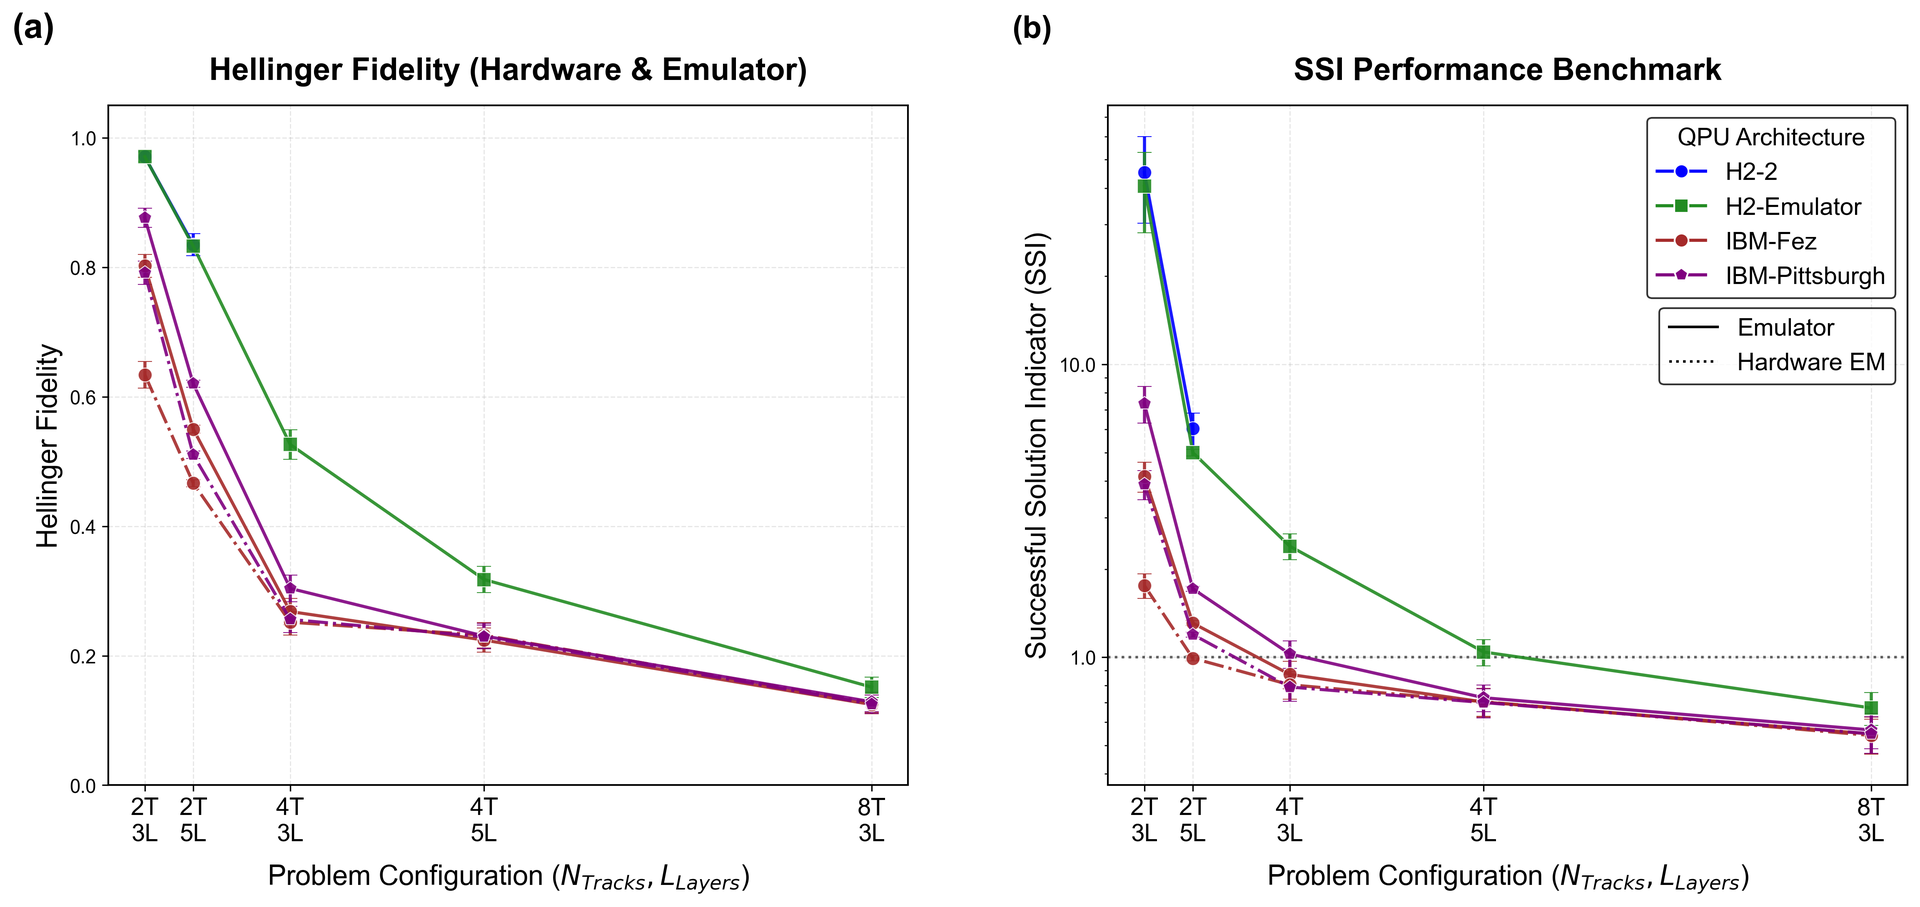
\includegraphics[width=0.92\textwidth,height=0.55\textheight,keepaspectratio]{figs/hardware_results.png}%
}{%
  \fbox{\parbox{0.6\textwidth}{\centering\vspace{1cm}
    \texttt{figs/hardware\_results.png} \\[2pt]
    \scriptsize drop the PNG into\\ \texttt{docs/reports/presentation\_planning/figs/}
    \vspace{1cm}}}%
}\\[1pt]
{\tiny Hellinger fidelity (left) and SSI (right) for 5 problem configurations across H2 (Quantinuum), IBM-Fez, IBM-Pittsburgh. Solid lines = ideal emulator (no noise). Dotted lines = noisy results with error mitigation (\textit{``EM''}): IBM lines are noise-model emulator + EM; the \textbf{H2-2 dotted point at 2T-3L is real Quantinuum hardware} --- the only physical-device data point. H2 (real + emulator) keeps SSI $>1$ except at 8T-3L; the IBM stack falls below SSI $=1$ from 4T-3L onward.}
\end{frame}

% =====================================================================
\section{Where we stand}

\begin{frame}{Open items --- 2 weeks to resubmission}
\footnotesize
\begin{tabular}{p{6.4cm} p{2.4cm} p{2.4cm}}
\toprule
\textbf{Item} & \textbf{Status} & \textbf{Owner} \\
\midrule
$\mathcal O(N)$ load-complexity paragraph & drafted & Xeno \\
HL-LHC throughput / classical-limit prose & TODO & TBD \\
``Outperform classical'' sentence & TODO & TBD \\
Realistic MC + SBT benchmark & running & Xeno \\
Quantum toy at high $n_{\mathrm{trk}}$ & running & George \\
Generality of the method (R2 Major 3) & TODO & TBD \\
Hardware run on a real device & uncertain & Xeno \\
Eq.\ 10 intermediate step & merge pending & Xeno \\
Error-mitigation paragraph & TODO & Xeno \\
Fake-rate expansion in Discussion & TODO & TBD \\
$n_s$ def, exhaustive-search ref, $r_i$ consistency & TODO & Xeno \\
Fault-tolerant scaling paragraph (R3) & TODO --- no expert & TBD \\
\bottomrule
\end{tabular}
\end{frame}

% =====================================================================
\begin{frame}{Schedule \& discussion}
\begin{itemize}
  \item Today: 29 April 2026. Resubmission window: $\sim$2 weeks.
  \item \textbf{Critical path:}
  \begin{itemize}
    \item Realistic MC benchmark (Xeno)
    \item Quantum toy at high $n_{\mathrm{trk}}$ (George)
    \item Classical-limits prose (R2 Major 1)
    \item Generality prose (R2 Major 3)
  \end{itemize}
  \item \textbf{Stretch:} fault-tolerant paragraph, error-mitigation prose, hardware on a real device.
  \item Discussion:
  \begin{itemize}
    \item Owners for the TBD rows
    \item Whether to push back the deadline if MC + hardware are not ready
    \item How to frame R2 Major 3 (full worked example or future work?)
  \end{itemize}
\end{itemize}
\end{frame}

% =====================================================================
\section{Extras}

\begin{frame}{Extra --- tracker A/B at the track level}
{\footnotesize Track-level metrics are not what the reviewers asked for, but they are useful context. With naive connected-components grouping, track efficiency collapses 99\% $\to$ 44\% between $n=300$ and $n=1000$. With a tracker that adds an angle check and module exclusivity (\emph{same} Hamiltonian, solver, threshold) it stays $\ge 99.96\%$ at every $n$.}
\begin{center}

\includegraphics[width=0.65\textwidth,height=0.55\textheight,keepaspectratio]{fig17_tracker_ab.pdf}
\end{center}
{\scriptsize The previous low track-level numbers were a tracker artefact, not a Hamiltonian limit.}
\end{frame}

\end{document}
